\documentclass[conference]{IEEEtran}
\IEEEoverridecommandlockouts
% The preceding line is only needed to identify funding in the first footnote. If that is unneeded, please comment it out.
\usepackage{cite}
\usepackage[hyphens]{url}
\usepackage{amsmath,amssymb,amsfonts}
\usepackage{algorithmic}
\usepackage{graphicx}
\usepackage{textcomp}
\usepackage{xcolor}
\usepackage{caption}
\captionsetup[table]{format=plain, font=small, labelformat=simple,labelsep=period}%
\usepackage{listings}
\usepackage{url}
\usepackage{float}
\def\BibTeX{{\rm B\kern-.05em{\sc i\kern-.025em b}\kern-.08em
    T\kern-.1667em\lower.7ex\hbox{E}\kern-.125emX}}
\begin{document}

\title{Investigating the Attack Surface of Hardware Wallets}

\author{\IEEEauthorblockN{1\textsuperscript{st} Talha Zia Muhammad Ali}
\IEEEauthorblockA{\textit{Master of Science in Power Engineering} \\
\textit{Technical University of Munich}\\
Munich, Germany \\
ge46tun@mytum.de}
}

\maketitle

%%%%%%%%%%%%%%%%%
%   Abstract    %
%%%%%%%%%%%%%%%%%

\begin{abstract}
The safety of cryptographic keys determines the security of cryptocurrencies. Using the innovative concept of blockchains, there is no 
straightforward way to tamper with online shared transaction ledger. Instead, attackers are interested in cryptographic keys which are 
necessary for managing cryptographic operations. Hardware wallets are considered the safest way to manage cryptographic key pairs.  

In this paper we are analyzing the vulnerabilities of hardware wallets in domain of supply chain, hardware, and software architecture. 
The analysis also inculcates both open-source code and closed source code hardware wallets. In addition, we are also assessing the attacks 
in terms of severity and scalability. In the end we are concluding that security of hardware wallet remains questionable in specific case 
of hardware vulnerabilities (side channel attacks), giving a broader picture of future challenges, making hardware wallets resistant to 
side channel attacks and introduction of social recovery features such that assets can be recovered in case of security breach.
\end{abstract}

\begin{IEEEkeywords}
Cryptocurrency, Blockchain, Hardware Wallet, Side Channel Attack, Deep Learning, Private Key.  
\end{IEEEkeywords}

%%%%%%%%%%%%%%%%%%%%%
%   Introduction    %
%%%%%%%%%%%%%%%%%%%%%

\section{Introduction}
Innovation of the Nakamoto consensus protocol gave compute nodes the opportunity to agree upon a shared ledger state in a trust-less 
network setup\cite{nakamoto2008bitcoin}. Almost all cryptocurrency, including Bitcoin, Ethereum, Bitcoin cash and Litecoin, make use 
of transparent ledger that is secured via block chain network. Without a central authority, everyone is allowed to connect a compute 
node to the network. Blockchains allow web services around blockchain nodes, making it feasible for users to interact with blockchains 
individually. When users send transactions to the blockchain, blockchain nodes order, include, and eventually append transactions to 
the blockchain state via consecutive blocks. Every transaction change the blockchain state at specific addresses\cite{julie2020blockchain}. 
Ownership of addresses is thereby managed by keys, which are in turn managed by user-controlled wallets.

With increasing value of assets stored at specific blockchain addresses, wallets controlling these addresses became targets for 
attackers \cite{arapinis2019formal}. Advent of software wallet attacks led to the development of hardware wallets which protect 
cryptographic keys in separate dedicated hardware devices. Even though hardware wallets protect users against many issues \cite{9014007}, 
hardware wallets are becoming a target itself. Getting a clear overview over recent hardware wallet attacks, their severity, complexity, 
and structure has found little attention in academic research. Hence, it is difficult to grasp state-of-the-art open challenges around 
hardware wallet security.

This work tries to clarify the vulnerabilities of hardware wallet keeping in view its hardware and software architecture. This work 
identifies two major open challenges, making hardware wallets resistant to side channel attacks and introduction of social recovery 
features such that assets can be recovered in case of security breach. These allow us to conclude that research in field of side channel 
data prediction of hardware wallet is paramount for security and reliability. This paper is constituted of six sections structured as 
follows: Section II provides the description of cryptocurrency fundamentals. Section III compares the scope of this research with 
previous similar work. Section IV covers security analysis of hardware wallets keeping in view recent case studies. The evaluation 
is covered in Section V, and section VI concludes with a conclusion and future challenges.

%%%%%%%%%%%%%%%%%%%%%%%%%
%   Background Study    %
%%%%%%%%%%%%%%%%%%%%%%%%%

\section{Background Study}
Cryptocurrency operations is managed and validated with asymmetric cryptography. The private key is used for generation of the corresponding 
public key and digital signatures on transaction requests as a proof of ownership and validation. The public key is used as an address besides 
providing its cryptographic purpose of operating in cryptographic algorithms\cite{huhmo2018blockchain}. Considering algorithm of asymmetric 
cryptography, the private key cannot be reconstructed from a public key or address. 

%%%%%%%%%%%%%%%%%%%%%%%%%
%   Blockchain Wallets  %
%%%%%%%%%%%%%%%%%%%%%%%%%

\subsection{Blockchain Wallets}
The wallet is a software that holds a private key and automates complex cryptography. The wallet accepts the requested transaction, signs it 
on your behalf using your private key, and sends it to a single blockchain node \cite{julie2020blockchain}. After validation with digital 
signature, transaction is entered by the miners on the transaction ledger.

%%%%%%%%%%%%%%%%%%%%%%%%%%%%%%%%%%%%%%%%
%   Blockchain Wallets Classification  %
%%%%%%%%%%%%%%%%%%%%%%%%%%%%%%%%%%%%%%%%

\subsection{Blockchain Wallets Classification}
Blockchain wallet or cryptocurrency wallets can be classified based on: \begin{itemize}
    \item Architecture (Standard or Hierarchical Deterministic)
    \item Functionality (Full Node or Simple Payment Verification)
    \item Accessibility (Hot Wallet or Cold Wallet)
\end{itemize} 
The following sub-paragraphs refer to the most common types of wallets: \\
\textbf{Standard Wallet:} creates a wallet.dat file that contains a private key\cite{shaik2020securing}. This file must be backed up by copying 
it to a safe digital storage. \\
\textbf{Hierarchical Deterministic (HD) Wallet:} generates an initial seed phrase, a string of common words that can be memorized instead 
of long confusing private key. \cite{ahamad2013survey}. \\ 
\textbf{Full Node Wallet:} holds full copy of blockchain for validating each and every transaction\cite{dai2018sblwt}. \\
\textbf{Simple Payment verification (SPV) Wallet:} relies on blockchain nodes that are connected to validate transactions making them faster 
and lesser memory allocation\cite{dai2018sblwt}. \\
\textbf{Hot wallet:} has internet access either via web service or a wallet installed on a device connected to internet such that there 
is a data traffic between host and web network\cite{das2019formal}. \\
\textbf{Cold wallet:} has no internet access in any way. Cold wallet is also referred to as Hardware wallet or Offline wallet\cite{das2019formal}.

%%%%%%%%%%%%%%%%%%%%%%%%%%%%%%%%%%%%%%%%%%%%%%%%%%%%
%   Advantages and Disadvantages of Hot Wallets    %
%%%%%%%%%%%%%%%%%%%%%%%%%%%%%%%%%%%%%%%%%%%%%%%%%%%%

\subsection{Advantages and Disadvantages of Software Wallets}
The web wallet or software wallet is a least secure option for storage since you are asking someone to hold your keys for you. Web wallets 
are highly convenient by providing high flexibility, allowing you to buy, sell or transfer cryptocurrency at any point and time\cite{jokic2019comparative}. 

%%%%%%%%%%%%%%%%%%%%%%%
%   Hardware Wallets  %
%%%%%%%%%%%%%%%%%%%%%%%

\subsection{Hardware Wallets}
Consider a computer, running a blockchain wallet, can get infected with malware, exposing private key to bad actors. This can be avoided by:
\begin{itemize}
    \item Computer is malware free (not practically possible)
    \item Dedicated single purpose simplified computer to run blockchain wallet
\end{itemize}
Hardware wallet is a computer that is stripped down of all logic except for a small screen, few buttons, and bare necessities for simple 
action of storing private key and signing transactions. Lesser complexity makes hardware wallet so dumb that it is theoretically impossible 
to hack or infect it with anything. Since Hardware wallet is such a simple device that can only store private key and sign transactions, 
it needs to be connected to a more sophisticated computer. A bridge software is required that can prepare transaction, communicate with 
hardware wallet, receive digitally signed transaction from hardware wallet and interact with block chain node via internet connectivity. 
Once a transaction request is received via the bridge software, hardware wallet signs it and sends it back to bridge software. Private key 
never leaves the hardware wallet. Minimalist and plain design enable them to be used with any computer without fear of being hacked or 
infected\cite{suratkar2020cryptocurrency}.  
\begin{figure}[t]
    \centering
    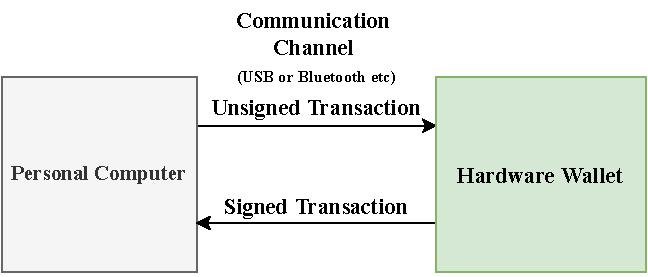
\includegraphics[width=70mm]{Figures/BD.pdf}
    \caption{Hardware Wallet Connectivity with PC}
    \label{fig1}
\end{figure}

%%%%%%%%%%%%%%%%%%%%
%   Related Work   %
%%%%%%%%%%%%%%%%%%%%

\section{Related Work}
Majority of previous research has focused on either the hardware wallet's specific attack surface (e.g., side channel attacks\cite{san2019side}, 
software attacks\cite{volotikin2018software}) or device-related attacks (TREZOR\cite{arapinis2019formal} or Keepkey\cite{almutairi2019usability}). 
However, a work presented at the USENIX Security Symposium in August 2021 \cite{pfeffer2021usability} provided an interesting perspective by 
listing potential attack surfaces for hardware wallets and evaluating them on all reputable hardware wallet devices. In addition, a study 
published in November 2021 \cite{dabrowski2021better} focuses on the characteristics and security engineering techniques (firmware attestation, 
software and hardware attestation). This seminar paper investigates the vulnerabilities of hardware wallets in the supply chain, hardware, and 
software architectural domains considering recent attacks. This work provides a fair summary as well as an interesting introduction paper to 
read. This study considers not just scholarly literature but also manufacturer's blog posts, giving readers a unique viewpoint on weaknesses 
as well as motivation for future research and development. 

%%%%%%%%%%%%%%%%%%%%%%%%%%%%%%%%%%%%%%%%%%%%%
%   Security Analysis of Hardware Wallets   %
%%%%%%%%%%%%%%%%%%%%%%%%%%%%%%%%%%%%%%%%%%%%%

\section{Security Analysis of Hardware Wallets}
Seed phrase is generated by device at random on initialization. Subsection A is a pre-analysis of the hardware wallets keeping in-view the hardware 
and software architecture. In subsections B, C and D, we go into deeper details of attacks. Attack surfaces are analyzed based on (i) supply chain 
attacks, (ii) hardware attacks, and (iii) software attacks. Under hardware attacks, this work investigates side channel and deep learning-based 
attacks. Software attacks are categorized on their scope towards application logic, general data attacks and communication attacks.

%%%%%%%%%%%%%%%%%%%%%%%%%%%%%%%%%%%%%%%%%%
%   Hardware and Software Architecture   %
%%%%%%%%%%%%%%%%%%%%%%%%%%%%%%%%%%%%%%%%%%

\subsection{Hardware and Software Architecture}
The hardware wallet can have multiple microcontrollers (MCU) and external peripherals. Hardware wallet software code can be fully open source or 
closed source. Primarily, hardware wallet provides (i) security enclave such that sensitive elements never leave the device, (ii) compact 
application programming Interface (API) comparable with microcontroller (MCU) persistent flash storage, and (iii) memory protection unit (MPU).\\     
% Block Diagram Dual MCU %
\begin{figure}[t]
    \centering
    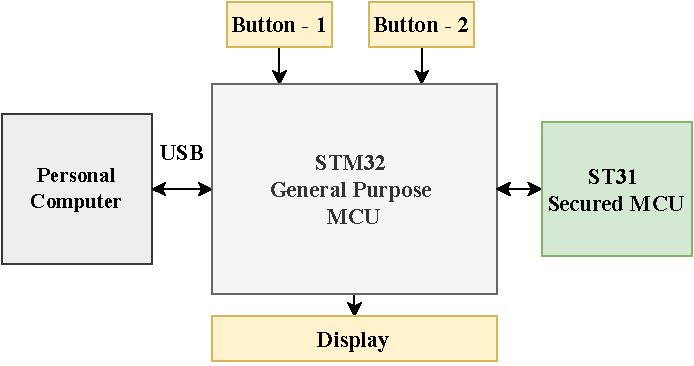
\includegraphics[width=75mm]{Figures/dualMCU.pdf}
    \caption{Hardware Architecture (dual chip design)}
    \label{fig2}
\end{figure}
\underline{Single Chip and Dual Chip Design:} Hardware wallets may use single general purpose microcontroller as in TREZOR \cite{arapinis2019formal} 
or a dual microcontroller as in Ledger Nano S \cite{suratkar2020cryptocurrency}. Single chip design is just a simple microcontroller, which is not 
meant to be very secure but fulfils the purpose (Fig \ref{fig2}). Dual chip design consists of a standard microcontroller, used as a proxy for 
managing the screen, button and connectivity and a secured microcontroller which handles secret elements (Fig \ref{fig3}). \\ 
\underline{Open Source or Closed Source:} Hardware wallet's software can either be open source or closed source. Open-source software has advantages 
such that anyone can audit the code, providing opportunities of improvements but also allowing attackers to exploit weaknesses \cite{san2019side}.

%%%%%%%%%%%%%%%%%%%%%%%%%%%
%   Supply Chain Attack   %
%%%%%%%%%%%%%%%%%%%%%%%%%%%

\subsection{Supply Chain Attack}
Supply chain attack means that device security has been compromised before its delivery to the end user. \\
\underline{Accessibility:} The attacker needs physical access to device either during transportation or attacker can buy a device from 
manufacturer's website, compromising preconfigured encryption and apply for device return as per manufacturer's policy. \\
\underline{Goal:} The goal of this attack is to know the seed phrase that user will use in future for cryptocurrency transfer either by 
malware injection or tempering device encryption chip. \\
\underline{Prevention:} Special holographic sticker is used as a proof that device is never tempered \cite{ledgerdata2}. This security 
check can be compromised without any traceability. Instead, most manufacturer offers device self authentication test on initialization, 
making sure that encryption chip is in original state \cite{volotikin2018software}. 

%%%%%%%%%%%%%%%%%%%%%%%%%%%%%%%%
%   Hardware Vulnerabilities   %
%%%%%%%%%%%%%%%%%%%%%%%%%%%%%%%%

\subsection{Hardware Vulnerabilities}
Most critical hardware vulnerability is side channel attack, an exploit that aims to gather system information by measuring hardware emission 
(power, electromagnetic emanations, acoustic emanations) or influencing program execution by exploiting its hardware (voltage glitching, 
temperature, clock frequency) \cite{san2019side}.\\
\underline{Accessibility:} Physical access to hardware is required. Side Channel attacks can be divided into two types: 
\begin{itemize}
    \item \textbf{Profiled Attacks}: Attacker must have access of two identical devices. Device A is evaluated, recording its behavior and a 
    data model is constructed, which is then used for device B whose sensitive information is unknown \cite{san2019side}. 
    \item \textbf{Non-Profiled Attacks}: Attacker has access of only a single closed target device allowing only limited number of side 
    channel traces\cite{timon2019non}.  
\end{itemize}
% Single Chip Hardware Wallets %
\begin{figure}[t]
    \centering
    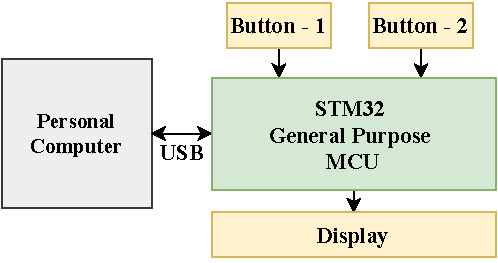
\includegraphics[width=60mm]{Figures/singleMCU.pdf}
    \caption{Hardware Architecture (single chip design)}
    \label{fig3}
\end{figure}
\underline{Supply Voltage Disturbance:} Supply voltage glitch forces hardware to give unpredictable behavior and PIN verification can be 
bypassed. The attack gives an attacker the opportunity to use the wallet and sign transactions with the wallet. PIN verification by microcontroller 
takes some time (order of milliseconds). Test is repeated multiple times with different offset (in microseconds) to accurately time the fault 
injection with critical instruction execution. \\
\underline{Power Consumption Analysis:} Encryption algorithm is a combination of mathematical operations (multiplication, addition etc.). Power 
consumption is different depending on the operation in progress. Precise measurements, multiple test points combined with statistics, algorithm of 
asymmetric encryption can be estimated and eventually estimating private key\cite{san2019side}. \\  
\underline{Deep Learning based side channel attacks:} Combining side channel attack traces with deep learning metrics, attacker can extract the 
bits of the keys used in the algorithms \cite{timon2019non}. First case study of machine learning in side channel attacks was done in 
2011 \cite{hospodar2011machine}. \\
\underline{Prevention:} Hardware Wallet are becoming resistant to external glitching such that device goes to reboot with a warning message but 
most of the time it is difficult to eliminate. Side channel attacks are tricky to defend.

%%%%%%%%%%%%%%%%%%%%%%%%%%%%%%%%
%   Software Vulnerabilities   %
%%%%%%%%%%%%%%%%%%%%%%%%%%%%%%%%

\subsection{Software Vulnerabilities}
Most common software attacks are flawed program design, buffer overflows or application programming interfaces vulnerabilities allowing unauthorized 
attacker to enter a system. Most common software vulnerabilities are:\\ 
\textbf{Data Layer Vulnerability:} Hardware wallets have memory protection units allowing APIs to access dedicated memory region 
\cite{suratkar2020cryptocurrency}. The goal of this attack is to somehow override memory protection unit and gain access of restricted 
memory region.\\
\underline{Attack:} Attacker can have access to device before initialization by user and a known seed is injected into the device. Attacker knows 
PIN code, installing a rogue API such that can break protected memory isolation.\\
\underline{Case Study:} Ledger hardware wallet had a bug causing memory protection unit (MPU) to be misconfigured, allowing attacker to read 16K 
of memory of supposed to be protected memory region\cite{ledgerdata1, ledgerdata2}. Similarly, a bug in Trezor hardware wallet allowed write to flash 
memory \cite{trezordata1}.\\
\textbf{Communication Layer Vulnerability:} Attacker can extract secret information from device via PC connectivity; commanding device to reveal 
or manipulate wallet secrets, change PIN even steel secret passphrase.\\
\underline{Attack:} Attack is triggered by malicious software on Computer and target device is unlocked either by user for normal operation or 
by the attacker. \\
\underline{Case Study:} This vulnerability was found in Keepkey Wallet\cite{keepkeystackoverflow} and Trezor Wallet such that data sent over USB 
interface can trigger a buffer overflow \cite{bufferoverflow} and USB leaked discarded memory \cite{usbleak}.\\
\textbf{Application Layer Vulnerabilities:} Attacker can take advantage of flawed program algorithm. Certain portion of device's firmware, bootloader 
and user data can get accessed during firmware update or rogue application installing.\\
\underline{Attack:} Attack is initiated by installing a rogue application or during firmware update.\\
\underline{Case Study:} The Ledger kernel had a bug in code; increasing number of system calls incorrectly validated pointer arguments, potentially 
allowing agents to read data belonging to the kernel or other agents. Also, during firmware update, user sensitive data is copied to RAM. Halting 
device at this point and with installing a rogue application that can set Debug Flag, contents of RAM are accessible over 
JTAG \cite{ledgerdata1, ledgerdata2}.   
\begin{table}[ht]
    \centering
    \caption{Hardware Wallets Attack Summary}
    \begin{tabular}[t]{|c|l|c|c|c|}
        \hline
        \textbf{\begin{tabular}[c]{@{}c@{}}Attack\\ Type\end{tabular}}   & \multicolumn{1}{c|}{\textbf{Goal}}                                                                                                                                                       & \textbf{Severity} & \textbf{Status} & \textbf{\begin{tabular}[c]{@{}c@{}}Ref.\end{tabular}}                                                                                                         \\ \hline
        \textbf{\begin{tabular}[c]{@{}c@{}}Supply \\ Chain\end{tabular}} & \begin{tabular}[c]{@{}l@{}}-Preconfiguration of \\ Seedphrase or PIN\end{tabular}                                                                                                        & Low               & Solved          & \begin{tabular}[c]{@{}c@{}}\cite{ledgerdata2}\\ \cite{volotikin2018software}\end{tabular}                                                                                   \\ \hline
        \textbf{Hardware}                                                & \begin{tabular}[c]{@{}l@{}}-Side Channel Attack\\  (Hardware measurements)\\ -Hardware analysis\\  (Deep Learning based)\\ -Hardware Glitching\\  (Voltage, Clock, Current)\end{tabular} & High              & Open            & \begin{tabular}[c]{@{}c@{}}\cite{san2019side}\\ \cite{timon2019non}\\ \cite{kocher1999differential}\\ \cite{hospodar2011machine}\end{tabular}                               \\ \hline
        \textbf{Software}                                                & \begin{tabular}[c]{@{}l@{}}-Device Memory Access\\ -Code injection to modify \\ encryption\\ -Device flawed algorithm\end{tabular}                                                       & High              & Open            & \begin{tabular}[c]{@{}c@{}}\cite{ledgerdata1}\\ \cite{ledgerdata2}\\ \cite{trezordata1}\\ \cite{keepkeystackoverflow}\\ \cite{bufferoverflow}\\ \cite{usbleak}\end{tabular} \\ \hline
    \end{tabular}
    \label{table:table1} 
\end{table}

%%%%%%%%%%%%%%%%%%
%   Evaluation   %
%%%%%%%%%%%%%%%%%%

\section{Evaluation}
Security analysis of hardware wallet is summarized in table \ref{table:table1}. In the early years of product development, supply chain attacks 
were profound but in later years, supply chain attacks are becoming less. Hardware vulnerabilities need physical access of the device. Side 
channel attacks are difficult to detect, tricky to defend and often do not leave any trace. Implementation of deep learning algorithm with side 
channel attacks have increased attack success rate. Software vulnerabilities need strong knowledge of software architecture and in majority cases, 
PIN code is also required for attack execution.    

%%%%%%%%%%%%%%%%%%%%%%%%%%%%%%%%%%
%   Conclusion and Future Work   %
%%%%%%%%%%%%%%%%%%%%%%%%%%%%%%%%%%

\section{Conclusion}

There are two main open challenges in making hardware wallets secure and dependable. First, with the increase in measurement sensitivity, it is 
possible to gather extremely detailed data about system when running, making side channel vulnerabilities hard to detect at product development 
stage. Even after its identification, its solution often requires re-designing of hardware architecture which in majority cases is not feasible. 
Second, there is a need of reviewing cryptographic operations of sending or receiving transactions such that transaction request by attacker can 
be reverted to the user, making assets recoverable in case of security breach. Hardware wallet security is a process of continuous evolution and 
further research, and development is required in these two domains.     

\bibliographystyle{ieeetr}
\bibliography{references}

\end{document}
